%
% This document contains the chapter about linear and non-linear devices.
%
% Copyright (C) 2003, 2004, 2005, 2006 Stefan Jahn <stefan@lkcc.org>
% Copyright (C) 2003, 2004, 2005, 2006
%               Michael Margraf <Michael.Margraf@alumni.TU-Berlin.DE>
%
% Permission is granted to copy, distribute and/or modify this document
% under the terms of the GNU Free Documentation License, Version 1.1
% or any later version published by the Free Software Foundation.
%


\chapter{Linear devices}
\label{sec:Ldevices}

As the MNA matrix is the y-parameter matrix of the whole circuit,
components that are defined by y-parameters can be easily inserted
by adding these parameters to the MNA matrix elements (so-called
'stamping').

\addvspace{12pt}

Components that cannot be defined by y-parameters need to add
additional columns and rows to the MNA matrix. Components
defined by z-parameters can be added in the following way
(example for a 2-port). It is easily extendable for any port
number.

\begin{equation}
\begin{bmatrix}
 . & .  &  1 & 0\\
 . & .  &  0 & 1\\
-1 &  0 & Z_{11} & Z_{12}\\
 0 & -1 & Z_{21} & Z_{22}
\end{bmatrix}
\cdot
\begin{bmatrix}
V_{1}\\
V_{2}\\
I_{in}\\
I_{out}
\end{bmatrix}
=
\begin{bmatrix}
I_{1}\\
I_{2}\\
0\\
0
\end{bmatrix}
\end{equation}

Components that are characterized by S-parameters (normalized to $Z_0$)
can be put into the MNA matrix by the following scheme (example for a
3-port). It is easily extendable for any port number.

\begin{equation}
\label{eqn:Sparam2mna}
\begin{bmatrix}
 . & . & .  &  1 & 0 & 0\\
 . & . & .  &  0 & 1 & 0\\
 . & . & .  &  0 & 0 & 1\\
S_{11}-1 &  S_{12} & S_{13} & Z_0\cdot (S_{11}+1) & Z_0\cdot S_{12} & Z_0\cdot S_{13}\\
S_{21} &  S_{22}-1 & S_{23} & Z_0\cdot S_{21} & Z_0\cdot (S_{22}+1) & Z_0\cdot S_{23}\\
S_{31} &  S_{32} & S_{33}-1 & Z_0\cdot S_{31} & Z_0\cdot S_{32} & Z_0\cdot (S_{33}+1)
\end{bmatrix}
\cdot
\begin{bmatrix}
V_{1}\\
V_{2}\\
V_{3}\\
I_{I1}\\
I_{I2}\\
I_{I3}
\end{bmatrix}
=
\begin{bmatrix}
I_{1}\\
I_{2}\\
I_{3}\\
0\\
0\\
0
\end{bmatrix}
\end{equation}


\section{Resistor}

For DC and AC simulation an ideal resistor with resistance $R$
yields:
\begin{equation}
Y = \dfrac{1}{R} \cdot
\begin{pmatrix}
 1 & -1 \\
-1 &  1 \\
\end{pmatrix}
\end{equation}

The noise correlation matrix at temperature $T$ yields:
\begin{equation}
(\underline{C}_Y) = \frac{4\cdot k\cdot T}{R} \cdot
\begin{pmatrix}
 1 & -1 \\
-1 &  1 \\
\end{pmatrix}
\end{equation}

The scattering parameters normalized to impedance $Z_0$
writes as follows.
\begin{equation}
S_{11} = S_{22} = \frac{R}{2\cdot Z_0+R} \\
\end{equation}
\begin{equation}
S_{12} = S_{21} = 1-S_{11} = \frac{2\cdot Z_0}{2\cdot Z_0+R}
\end{equation}

Being on temperature $T$, the noise wave correlation matrix
writes as follows.
\begin{equation}
(\underline{C}) = k\cdot T\cdot\frac{4\cdot R\cdot Z_0}{(2\cdot Z_0+R)^2}\cdot
\begin{pmatrix}
   1 & -1\\
  -1 &  1\\
\end{pmatrix}
\end{equation}

The noise wave correlation matrix of a parallel resistor with resistance $R$
writes as follows.
\begin{equation}
(\underline{C}) = k\cdot T\cdot\frac{4\cdot R\cdot Z_0}{(2\cdot R+Z_0)^2}\cdot
\begin{pmatrix}
  1 & 1\\
  1 & 1\\
\end{pmatrix}
\end{equation}

The noise wave correlation matrix of a grounded resistor with resistance $R$
is a matrix consisting of one element and writes as follows.
\begin{equation}
(\underline{C}) = k\cdot T\cdot\frac{4\cdot R\cdot Z_0}{(R+Z_0)^2}
\end{equation}


\section{Capacitor}

During DC simulation the capacitor is an open circuit. Thus, its MNA
entries are all zero.

\addvspace{12pt}

During AC simulation the y-parameter matrix of an ideal capacitor
with the capacitance $C$ writes as follows.
\begin{equation}
Y =
\begin{bmatrix}
+j\omega C & -j\omega C\\
-j\omega C & +j\omega C\\
\end{bmatrix}
\end{equation}

The scattering parameters (normalized to $Z_0$) of an ideal capacitor
with capacitance $C$ writes as follows.
\begin{equation}
S_{11} = S_{22} = \frac{1}{2\cdot Z_0\cdot j\omega C+1} \\
\end{equation}
\begin{equation}
S_{12} = S_{21} = 1-S_{11}
\end{equation}

An ideal capacitor is noise free. Its noise correlation matrices
are, therefore, zero.


\section{Inductor}

During DC simulation an inductor is a short circuit, thus, its
MNA matrix entries need an additional row and column.
\begin{equation}
\begin{bmatrix}
. & . & +1\\
. & . & -1\\
+1 & -1 & 0\\
\end{bmatrix}
\cdot
\begin{bmatrix}
V_1\\
V_2\\
I_{br}\\
\end{bmatrix}
=
\begin{bmatrix}
I_1\\
I_2\\
0
\end{bmatrix}
\end{equation}

During AC simulation the Y-parameter matrix of an ideal inductor
with the inductance $L$ writes as follows.
\begin{equation}
Y =
\begin{bmatrix}
+\dfrac{1}{j\omega L} & -\dfrac{1}{j\omega L}\\
-\dfrac{1}{j\omega L} & +\dfrac{1}{j\omega L}\\
\end{bmatrix}
\end{equation}

The scattering parameters of an ideal inductor with inductance $L$
writes as follows.
\begin{equation}
S_{11} = S_{22} = \frac{j\omega L}{2\cdot Z_0 + j\omega L} \\
\end{equation}
\begin{equation}
S_{12} = S_{21} = 1-S_{11}
\end{equation}

An ideal inductor is noise free.


\section{DC Block}

A DC block is a capacitor with an infinite capacitance. During DC
simulation the DC block is an open circuit. Thus, its MNA
entries are all zero.

\addvspace{12pt}

The MNA matrix entries of a DC block correspond to an ideal short
circuit during AC analysis which is modeled by a voltage source with
zero voltage.
\begin{equation}
\begin{bmatrix}
. & . & +1\\
. & . & -1\\
+1 & -1 & 0\\
\end{bmatrix}
\cdot
\begin{bmatrix}
V_1\\
V_2\\
I_{br}\\
\end{bmatrix}
=
\begin{bmatrix}
I_1\\
I_2\\
0
\end{bmatrix}
\end{equation}

The scattering parameters writes as follows.
\begin{equation}
\begin{pmatrix}
S
\end{pmatrix}
=
\begin{pmatrix}
0 & 1\\
1 & 0\\
\end{pmatrix}
\end{equation}

A DC block is noise free. A model for transient simulation does not
exist. It is common practice to model it as a capacitor with finite
capacitance whose value is entered by the user.


\section{DC Feed}

A DC feed is an inductor with an infinite inductance. The MNA
matrix entries of a DC feed correspond to an ideal short
circuit during DC analysis:
\begin{equation}
\begin{bmatrix}
. & . & +1\\
. & . & -1\\
+1 & -1 & 0\\
\end{bmatrix}
\cdot
\begin{bmatrix}
V_1\\
V_2\\
I_{br}\\
\end{bmatrix}
=
\begin{bmatrix}
I_1\\
I_2\\
0
\end{bmatrix}
\end{equation}

During AC simulation the DC feed is an open circuit. Thus, its MNA
entries are all zero.

\addvspace{12pt}

The scattering parameters writes as follows.
\begin{equation}
\begin{pmatrix}
S
\end{pmatrix}
=
\begin{pmatrix}
1 & 0\\
0 & 1\\
\end{pmatrix}
\end{equation}

A DC feed is noise free. A model for transient simulation does not
exist. It is common practice to model it as an inductor with finite
inductance whose value is entered by the user.


\section{Bias T}

An ideal bias t is a combination of a DC block and a DC feed
(fig. \ref{fig:biast}). During DC simulation the MNA matrix
of an ideal bias t writes as follows:

\begin{equation}
\begin{bmatrix}
 . & . & .  &  0\\
 . & . & .  &  1\\
 . & . & .  & -1\\
 0 & 1 & -1 &  0
\end{bmatrix}
\cdot
\begin{bmatrix}
V_{1}\\
V_{2}\\
V_{3}\\
I_{out}
\end{bmatrix}
=
\begin{bmatrix}
I_{1}\\
I_{2}\\
I_{3}\\
0
\end{bmatrix}
\end{equation}

\begin{figure}[ht]
\begin{center}
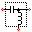
\includegraphics[width=3.5cm]{biast}
\end{center}
\caption{bias t}
\label{fig:biast}
\end{figure}
\FloatBarrier

The MNA entries of the bias t during AC analysis write as
follows.
\begin{equation}
\begin{bmatrix}
 . & . & .  & -1\\
 . & . & .  &  1\\
 . & . & .  &  0\\
-1 & 1 & 0  &  0
\end{bmatrix}
\cdot
\begin{bmatrix}
V_{1}\\
V_{2}\\
V_{3}\\
I_{out}
\end{bmatrix}
=
\begin{bmatrix}
I_{1}\\
I_{2}\\
I_{3}\\
0
\end{bmatrix}
\end{equation}

The scattering parameters writes as follows.

\begin{equation}
\begin{pmatrix}
S
\end{pmatrix}
=
\begin{pmatrix}
0 & 1 & 0\\
1 & 0 & 0\\
0 & 0 & 1\\
\end{pmatrix}
\end{equation}

A bias t is noise free. A model for transient simulation does not
exist. It is common practice to model it as an inductor and a
capacitance with finite values which are entered by the user.


\section{Transformer}

The two winding ideal transformer, as shown in fig.
\ref{fig:trafo}, is determined by the following equation which
introduces one more unknown in the MNA matrix.

\begin{figure}[ht]
\begin{center}
\includegraphics[width=4cm]{actrafo}
\end{center}
\caption{ideal two winding transformer}
\label{fig:trafo}
\end{figure}
\FloatBarrier

\begin{equation}
T\cdot\left(V_{2} - V_{3}\right) = V_{1} -V_{4}
\quad \rightarrow \quad
V_{1} - T\cdot V_{2} + T\cdot V_{3} - V_{4} = 0
\label{eq:trafo}
\end{equation}

The new unknown variable $I_{t}$ must be considered by the four
remaining simple equations.

\begin{equation}
I_{1} = -I_{t} \quad I_{2} = T\cdot I_{t} \quad I_{3} = -T\cdot I_{t} \quad I_{4} = I_{t}
\end{equation}

And in matrix representation this is for DC and for AC simulation:
\begin{equation}
\begin{bmatrix}
.&.&.&.& -1\\
.&.&.&.& T\\
.&.&.&.& -T\\
.&.&.&.& 1\\
1 & -T & T & -1 & 0
\end{bmatrix}
\cdot
\begin{bmatrix}
V_{1}\\
V_{2}\\
V_{3}\\
V_{4}\\
I_{t}
\end{bmatrix}
=
\begin{bmatrix}
I_{1}\\
I_{2}\\
I_{3}\\
I_{4}\\
0
\end{bmatrix}
\end{equation}

It is noticeable that the additional row (part of the C matrix) and the
corresponding column (part of the B matrix) are transposed to each
other.  When considering the turns ratio $T$ being complex introducing
an additional phase the transformer can be used as phase-shifting
transformer.  Both the vectors must be conjugated complex transposed
in this case.

\addvspace{12pt}

Using the port numbers depicted in fig. \ref{fig:trafo}, the
scattering parameters of an ideal transformer with voltage
transformation ratio $T$ (number of turns) writes as follows.

\begin{equation}
S_{14} = S_{22} = S_{33} = S_{41} = \frac{1}{T^2+1}
\end{equation}
\begin{equation}
S_{12} = -S_{13} = S_{21} = -S_{24} = -S_{31} = S_{34} = -S_{42} = S_{43} = T\cdot S_{22}
\end{equation}
\begin{equation}
S_{11} = S_{23} = S_{32} = S_{44} = T\cdot S_{12}
\end{equation}

An ideal transformer is noise free.


\section{Symmetrical transformer}

The ideal symmetrical transformer, as shown in fig.
\ref{fig:strafo}, is determined by the following equations which
introduce two more unknowns in the MNA matrix.

\begin{figure}[ht]
\begin{center}
\includegraphics[width=4cm]{acstrafo}
\end{center}
\caption{ideal three winding transformer}
\label{fig:strafo}
\end{figure}
\FloatBarrier

\begin{equation}
T_{1}\cdot\left(V_{2} - V_{3}\right) = V_{1} - V_{6}
\quad \rightarrow \quad
V_{1} - T_{1}\cdot V_{2} + T_{1}\cdot V_{3} - V_{6} = 0
\end{equation}
\begin{equation}
T_{2}\cdot\left(V_{2} - V_{3}\right) = V_{5} - V_{4}
\quad \rightarrow \quad
- T_{2}\cdot V_{2} + T_{2}\cdot V_{3} - V_{4} + V_{5} = 0
\label{eq:acstrafo}
\end{equation}

The new unknown variables $I_{T1}$ and $I_{T2}$ must be considered by
the six remaining simple equations.
\begin{equation}
I_{2} = T_{1}\cdot I_{T1} + T_{2}\cdot I_{T2} \quad I_{3} = -T_{1}\cdot I_{T1} - T_{2}\cdot I_{T2}
\end{equation}
\begin{equation}
I_{1} = -I_{T1} \quad I_{4} = I_{T2} \quad I_{5} = -I_{T2} \quad I_{6} = I_{T1}
\end{equation}

The matrix representation needs to be augmented by two more new rows
and their corresponding columns. For DC and AC simulation it is:
\begin{equation}
\begin{bmatrix}
.&.&.&.&.&.& -1 & 0\\
.&.&.&.&.&.& T_{1} & T_{2}\\
.&.&.&.&.&.& -T_{1} & -T_{2}\\
.&.&.&.&.&.& 0 & 1\\
.&.&.&.&.&.& 0 & -1\\
.&.&.&.&.&.& 1 & 0\\
1 & -T_{1} & T_{1} & 0 & 0 & -1 & 0 & 0\\
0 & -T_{2} & T_{2} & -1 & 1 & 0 & 0 & 0
\end{bmatrix}
\cdot
\begin{bmatrix}
V_{1}\\
V_{2}\\
V_{3}\\
V_{4}\\
V_{5}\\
V_{6}\\
I_{T1}\\
I_{T2}
\end{bmatrix}
=
\begin{bmatrix}
I_{1}\\
I_{2}\\
I_{3}\\
I_{4}\\
I_{5}\\
I_{6}\\
0\\
0
\end{bmatrix}
\end{equation}

Using the port numbers depicted in fig. \ref{fig:strafo}, the
scattering parameters of an ideal, symmetrical transformer with
voltage transformation ratio (number of turns) $T_1$ and $T_2$,
respectively, writes as follows.

\begin{equation}
denom = 1+T_1^2+T_2^2
\end{equation}
\begin{eqnarray}
S_{11} = S_{66} = \frac{T_1^2}{denom}  &  \qquad S_{16} = S_{61} = 1-S_{11} \\
S_{44} = S_{55} = \frac{T_2^2}{denom}  &  \qquad S_{45} = S_{54} = 1-S_{44} \\
S_{22} = S_{33} = \frac{1}{denom}  &  \qquad S_{23} = S_{32} = 1-S_{22}
\end{eqnarray}
\begin{equation}
S_{12} = S_{21} = -S_{13} = -S_{31} = -S_{26} = -S_{62} = S_{36} = S_{63}
       = \frac{T_1}{denom}
\end{equation}
\begin{equation}
-S_{24} = -S_{42} = S_{25} = S_{52} = S_{34} = S_{43} = -S_{35} = -S_{53}
       = \frac{T_2}{denom}
\end{equation}
\begin{equation}
-S_{14} = -S_{41} = S_{15} = S_{51} = S_{46} = S_{64} = -S_{56} = -S_{65}
       = \frac{T_1\cdot T_2}{denom}
\end{equation}

An ideal symmetrical transformer is noise free.


\section{Non-ideal transformer}

Many simulators support non-ideal transformers (e.g. mutual inductor
in SPICE).  An often used model consists of finite inductances and an
imperfect coupling (straw inductance).  This model has three
parameters: Inductance of the primary coil $L_1$, inductance of the
secondary coil $L_2$ and the coupling factor $k=0...1$.

\addvspace{12pt}

This model can be replaced by the equivalent circuit depicted in
figure \ref{fig:nitrafo}.  The values are calculated as follows.

\begin{align}
\textrm{turn ratio:} & \qquad  T = \sqrt{\frac{L_1}{L_2}}\\
\textrm{mutual inductance:}  & \qquad M = k\cdot L_1\\
\textrm{primary inductance:}  & \qquad L_{1,new} = L_1 - M = L_1\cdot (1-k)\\
\textrm{secondary inductance:}  & \qquad L_{2,new} = L_2 - \frac{M}{T^2} = L_2\cdot (1-k)
\end{align}

\begin{figure}[ht]
\begin{center}
\includegraphics[width=7.5cm]{nitrafo}
\end{center}
\caption{equivalent circuit of non-ideal transformer}
\label{fig:nitrafo}
\end{figure}
\FloatBarrier

The Y-parameters of this component are:
\begin{align}
Y_{11} = Y_{44} = -Y_{41} = -Y_{14} &= \frac{1}{j\omega\cdot L_1\cdot (1-k^2)}\\
Y_{22} = Y_{33} = -Y_{23} = -Y_{32} &= \frac{1}{j\omega\cdot L_2\cdot (1-k^2)}\\
Y_{13} = Y_{31} = Y_{24} = Y_{42} = -Y_{12} = -Y_{21} = -Y_{34} = -Y_{43} &=
  \frac{k}{j\omega\cdot\sqrt{L_1\cdot L_2}\cdot (1-k^2)}
\end{align}

Furthermore, its S-parameters are:
\begin{equation}
D = (k^2 - 1) \cdot \dfrac{\omega^2\cdot L_1\cdot L_2}{2\cdot Z_0} +
    j\omega L_1 + j\omega L_2 + 2\cdot Z_0
\end{equation}
\begin{equation}
S_{14} = S_{41} = \frac{j\omega L_2 + 2\cdot Z_0}{D}
\end{equation}
\begin{equation}
S_{11} = S_{44} = 1 - S_{14}
\end{equation}
\begin{equation}
S_{23} = S_{32} = \frac{j\omega L_1 + 2\cdot Z_0}{D}
\end{equation}
\begin{equation}
S_{22} = S_{33} = 1 - S_{23}
\end{equation}
\begin{equation}
S_{12} = -S_{13} = S_{21} = -S_{24} = -S_{31} = S_{34} = -S_{42} = S_{43} =
         \dfrac{j\omega\cdot k \cdot\sqrt{L_1\cdot L_2}}{D}
\end{equation}

Also including an ohmic resistance $R_1$ and $R_2$ for each coil,
leads to the following Y-parameters:
\begin{align}
Y_{11} = Y_{44} = -Y_{41} = -Y_{14} &
  = \dfrac{1}{j\omega\cdot L_1\cdot \left(1-k^2\cdot\dfrac{j\omega L_2}{j\omega L_2 + R_2}\right) + R_1}\\
Y_{22} = Y_{33} = -Y_{23} = -Y_{32} &
  = \dfrac{1}{j\omega\cdot L_2\cdot \left(1-k^2\cdot\dfrac{j\omega L_1}{j\omega L_1 + R_1}\right) + R_2}\\
Y_{13} = Y_{31} = Y_{24} = Y_{42} = -Y_{12} &= -Y_{21} = -Y_{34} = -Y_{43} =
  k\cdot\frac{j\omega\sqrt{L_1\cdot L_2}}{j\omega\cdot L_2 + R_2}\cdot Y_{11}
\end{align}

Building the S-parameters leads to too large equations. Numerically
converting the Y-parameters into S-parameters is therefore recommended.

\addvspace{12pt}

The MNA matrix entries during DC analysis and the noise correlation
matrices of this transformer are:
\begin{equation}
(\underline{Y}) =
\begin{pmatrix}
 1/R_1 & 0 & 0 & -1/R_1 \\
 0 &  1/R_2 & -1/R_2 & 0 \\
 0 & -1/R_2 &  1/R_2 & 0 \\
-1/R_1 & 0 & 0 &  1/R_1 \\
\end{pmatrix}
\end{equation}

\begin{equation}
(\underline{C}_Y) = 4\cdot k\cdot T\cdot
\begin{pmatrix}
 1/R_1 & 0 & 0 & -1/R_1 \\
 0 &  1/R_2 & -1/R_2 & 0 \\
 0 & -1/R_2 &  1/R_2 & 0 \\
-1/R_1 & 0 & 0 &  1/R_1 \\
\end{pmatrix}
\end{equation}

\begin{equation}
(\underline{C}_S) = 4\cdot k\cdot T\cdot Z_0\cdot
\begin{pmatrix}
 \tfrac{R_1}{(2\cdot Z_0 + R_1)^2} & 0 & 0 & -\tfrac{R_1}{(2\cdot Z_0 + R_1)^2} \\
 0 &  \tfrac{R_2}{(2\cdot Z_0 + R_2)^2} & -\tfrac{R_2}{(2\cdot Z_0 + R_2)^2} & 0 \\
 0 & -\tfrac{R_2}{(2\cdot Z_0 + R_2)^2} &  \tfrac{R_2}{(2\cdot Z_0 + R_2)^2} & 0 \\
-\tfrac{R_1}{(2\cdot Z_0 + R_1)^2} & 0 & 0 &  \tfrac{R_1}{(2\cdot Z_0 + R_1)^2} \\
\end{pmatrix}
\end{equation}

\addvspace{12pt}

A transformer with three coupled inductors has three coupling factors
$k_{12}$, $k_{13}$ and $k_{23}$.  Its Y-parameters write as follows
(port numbers are according to figure \ref{fig:strafo}).

\begin{gather}
A = j\omega\cdot (1 - k_{12}^2 - k_{13}^2 - k_{23}^2 + 2\cdot k_{12}\cdot k_{13}\cdot k_{23} ) \\
Y_{11} = Y_{66} = -Y_{16} = -Y_{61} = \dfrac{1-k_{23}^2}{L_1\cdot A} \\
Y_{22} = Y_{33} = -Y_{23} = -Y_{32} = \dfrac{1-k_{12}^2}{L_3\cdot A} \\
Y_{44} = Y_{55} = -Y_{45} = -Y_{54} = \dfrac{1-k_{13}^2}{L_2\cdot A} \\
Y_{12} = Y_{21} = Y_{36} = Y_{63} = -Y_{13} = -Y_{31} = -Y_{26} = -Y_{62}
   = \dfrac{k_{12}\cdot k_{23} - k_{13}}{\sqrt{L_1\cdot L_3}\cdot A} \\
Y_{15} = Y_{51} = Y_{46} = Y_{64} = -Y_{14} = -Y_{41} = -Y_{56} = -Y_{65}
   = \dfrac{k_{13}\cdot k_{23} - k_{12}}{\sqrt{L_1\cdot L_2}\cdot A} \\
Y_{25} = Y_{52} = Y_{43} = Y_{34} = -Y_{24} = -Y_{42} = -Y_{53} = -Y_{35}
   = \dfrac{k_{12}\cdot k_{13} - k_{23}}{\sqrt{L_2\cdot L_3}\cdot A}
\end{gather}

A more general approach for coupled inductors can be obtained by
using the induction law:

\begin{equation}
V_L = j\omega L\cdot I_L + j\omega\cdot \sum_{n=1}^N k_n\cdot\sqrt{L\cdot L_n}\cdot I_{L,n}
\end{equation}
where $V_L$ and $I_L$ is the voltage across and the current through
the inductor, respectively.  $L$ is its inductance.  The inductor is
coupled with $N$ other inductances $L_n$.  The corresponding coupling
factors are $k_n$ and $I_{L,n}$ are the currents through the inductors.

\addvspace{12pt}

Realizing this approach with the MNA matrix is straight forward: Every
inductance $L$ needs an additional matrix row.  The corresponding
element in the $D$ matrix is $j\omega L$.  If two inductors are
coupled the cross element in the $D$ matrix is $j\omega
k\cdot\sqrt{L_1\cdot L_2}$.  For two coupled inductors this yields:

\begin{equation}
\begin{bmatrix}
. & . & . & . & +1 &  0\\
. & . & . & . & -1 &  0\\
. & . & . & . &  0 & +1\\
. & . & . & . &  0 & -1\\
+1 & -1 & 0 & 0 & j\omega L_1 & j\omega k\cdot\sqrt{L_1\cdot L_2} \\
0 & 0 & +1 & -1 & j\omega k\cdot\sqrt{L_1\cdot L_2} & j\omega L_2 \\
\end{bmatrix}
\cdot
\begin{bmatrix}
V_1\\
V_2\\
V_3\\
V_4\\
I_{br1}\\
I_{br2}\\
\end{bmatrix}
=
\begin{bmatrix}
I_1\\
I_2\\
I_3\\
I_4\\
0
\end{bmatrix}
\end{equation}

Obviously, this approach has an advantage: It also works for zero
inductances and for unity coupling factors. It has the disadvantage
that it enlarges the MNA matrix.


\section{Attenuator}
\label{sec:dc_attenuator}

The ideal attenuator with (power) attenuation $L$ is frequency
independent and the model is valid for DC and for AC simulation.
It is determined by the following Z parameters.

\begin{equation}
Z_{11} = Z_{22} = Z_{ref}\cdot\frac{L+1}{L-1}
\end{equation}
\begin{equation}
Z_{12} = Z_{21} = Z_{ref}\cdot\frac{2\cdot\sqrt{L}}{L-1}
\end{equation}

The Z parameter representation is not very practical as new lines
in the MNA matrix have to be added. More useful are the Y parameters.

\begin{equation}
\frac{1}{Z_{ref}\cdot (L-1)}\cdot
\begin{bmatrix}
 L+1            & -2\cdot\sqrt{L} \\
-2\cdot\sqrt{L} & L+1
\end{bmatrix}
\cdot
\begin{bmatrix}
V_{1}\\
V_{2}
\end{bmatrix}
=
\begin{bmatrix}
I_{1}\\
I_{2}
\end{bmatrix}
\end{equation}

Attenuator with (power) attenuation $L$, reference impedance $Z_{ref}$
and temperature $T$:
\begin{equation}
(\underline{C}_Y) = 4\cdot k\cdot T\cdot \textrm{Re}\left(\underline{Y}\right)
 = \frac{4\cdot k\cdot T}{Z_{ref}\cdot (L-1)} \cdot
\begin{pmatrix}
 L+1            & -2\cdot\sqrt{L} \\
-2\cdot\sqrt{L} &  L+1 \\
\end{pmatrix}
\end{equation}

The scattering parameters and noise wave correlation matrix of an
ideal attenuator with (power) attenuation $L$ (loss) (or power gain
$G=1/L$) in reference to the impedance $Z_{ref}$ writes as follows.

\begin{equation}
S_{11} = S_{22} = \frac{r\cdot(L-1)}{L-r^2} = \frac{r\cdot(1-G)}{1-r^2\cdot G}
\end{equation}
\begin{equation}
S_{12} = S_{21} = \frac{\sqrt{L}\cdot(1-r^2)}{L-r^2} = \frac{\sqrt{G}\cdot(1-r^2)}{1-r^2\cdot G}
\end{equation}

\begin{equation}
(\underline{C}) = k\cdot T\cdot\frac{(L-1)\cdot(r^2-1)}{(L-r^2)^2}\cdot
\begin{pmatrix}
  -r^2-L           & 2\cdot r\sqrt{L}\\
  2\cdot r\sqrt{L} & -r^2-L\\
\end{pmatrix}
\end{equation}
with
\begin{equation}
r=\frac{Z_{ref}-Z_0}{Z_{ref}+Z_0}
\end{equation}


\section{Amplifier}

An ideal amplifier increases signal strength from input to output and
blocks all signals flowing into the output.  
The ideal amplifier is an isolator with voltage gain $G$ and is
determined by the following Z or Y parameters (valid for DC and
AC simulation).

\begin{equation}
Z_{11} = Z_1  \qquad
Z_{12} = 0
\end{equation}
\begin{equation}
Z_{21} = 2\cdot\sqrt{Z_1\cdot Z_2}\cdot G  \qquad
Z_{22} = Z_2
\end{equation}
\begin{equation}
Y_{11} = \frac{1}{Z_1}  \qquad
Y_{12} = 0
\end{equation}
\begin{equation}
Y_{21} = -\frac{2\cdot G}{\sqrt{Z_1\cdot Z_2}}  \qquad
Y_{22} = \frac{1}{Z_2}
\end{equation}

With the reference
impedance of the input $Z_1$ and the one of the output $Z_2$ and the
voltage amplification $G$, the scattering parameters of an ideal
amplifier write as follows.

\begin{equation}
S_{11} = \frac{Z_1-Z_0}{Z_1+Z_0}
\end{equation}
\begin{equation}
S_{12} = 0
\end{equation}
\begin{equation}
S_{22} = \frac{Z_2-Z_0}{Z_2+Z_0}
\end{equation}
\begin{equation}
S_{21} = \frac{4\cdot Z_0\cdot\sqrt{Z_1\cdot Z_2}\cdot G}{(Z_1+Z_0)\cdot(Z_2+Z_0)}
\end{equation}


\section{Isolator}

An isolator is a one-way two-port, transporting incoming waves
lossless from the input (port 1) to the output (port 2), but dissipating
all waves flowing into the output.
The ideal isolator with reference impedances $Z_1$ (input) and $Z_2$
(output) is determined by the following Z parameters (for DC and
AC simulation).

\begin{equation}
Z_{11} = Z_1  \qquad
Z_{12} = 0
\end{equation}
\begin{equation}
Z_{21} = 2\cdot\sqrt{Z_1\cdot Z_2}  \qquad
Z_{22} = Z_2
\end{equation}

A more useful MNA representation is with Y parameters.

\begin{equation}
\begin{bmatrix}
 \dfrac{1}{Z_1} & 0 \\
 \dfrac{-2}{\sqrt{Z_1\cdot Z_2}} & \dfrac{1}{Z_2}
\end{bmatrix}
\cdot
\begin{bmatrix}
V_{1}\\
V_{2}
\end{bmatrix}
=
\begin{bmatrix}
I_{1}\\
I_{2}
\end{bmatrix}
\end{equation}

Isolator with reference impedance $Z_1$ (input) and $Z_2$ (output) and
temperature $T$:
\begin{equation}
(\underline{C}_Y) = 4\cdot k\cdot T\cdot
\begin{pmatrix}
 \dfrac{1}{Z_1} & 0 \\
 \dfrac{-2}{\sqrt{Z_1\cdot Z_2}} &  \dfrac{1}{Z_2} \\
\end{pmatrix}
\end{equation}

With the reference impedance of the
input $Z_1$ and the one of the output $Z_2$, the scattering parameters
of an ideal isolator writes as follows.

\begin{equation}
S_{11} = \frac{Z_1-Z_0}{Z_1+Z_0}
\end{equation}
\begin{equation}
S_{12} = 0
\end{equation}
\begin{equation}
S_{22} = \frac{Z_2-Z_0}{Z_2+Z_0}
\end{equation}
\begin{equation}
S_{21} = \sqrt{1-(S_{11})^2}\cdot\sqrt{1-(S_{22})^2}
\end{equation}

Being on temperature $T$, the noise wave correlation matrix of an
ideal isolator with reference impedance $Z_1$ and $Z_2$ (input and
output) writes as follows.

\begin{equation}
(\underline{C}) = \frac{4\cdot k\cdot T\cdot Z_0}{(Z_1+Z_0)^2}\cdot
\begin{pmatrix}
  Z_1 & \sqrt{Z_1\cdot Z_2}\cdot\dfrac{Z_0-Z_1}{Z_0+Z_2}\\
  \sqrt{Z_1\cdot Z_2}\cdot\dfrac{Z_0-Z_1}{Z_0+Z_2} & Z_2\cdot\left(\dfrac{Z_1-Z_0}{Z_2+Z_0}\right)^2\\
\end{pmatrix}
\end{equation}


\section{Circulator}
\label{sec:CirculatorSparameter}

A circulator is a 3-port device, transporting incoming waves lossless
from port 1 to port 2, from port 2 to port 3 and from port 3 to port
1.  In all other directions, there is no energy flow.
The ideal circulator cannot be characterized with Z or Y parameters,
because their values are partly infinite.  But implementing with S
parameters is practical (see equation \ref{eqn:Sparam2mna}).

\addvspace{12pt}

With the
reference impedances $Z_1$, $Z_2$ and $Z_3$ for the ports 1, 2 and 3
the scattering matrix of an ideal circulator writes as follows.

\begin{equation}
denom = 1-r_1\cdot r_2\cdot r_3
\end{equation}
\begin{equation}
r_1 = \frac{Z_0-Z_1}{Z_0+Z_1} \qquad,\qquad 
r_2 = \frac{Z_0-Z_2}{Z_0+Z_2} \qquad,\qquad 
r_3 = \frac{Z_0-Z_3}{Z_0+Z_3}
\end{equation}
\begin{equation}
S_{11} = \frac{r_2\cdot r_3 - r_1}{denom} \qquad,\qquad
S_{22} = \frac{r_1\cdot r_3 - r_2}{denom} \qquad,\qquad 
S_{33} = \frac{r_1\cdot r_2 - r_3}{denom}
\end{equation}
\begin{equation}
S_{12} = \sqrt{\frac{Z_2}{Z_1}}\cdot\frac{Z_1+Z_0}{Z_2+Z_0}\cdot\frac{r_3\cdot(1-r_1^2)}{denom}
\qquad,\qquad 
S_{13} = \sqrt{\frac{Z_3}{Z_1}}\cdot\frac{Z_1+Z_0}{Z_3+Z_0}\cdot\frac{1-r_1^2}{denom}
\end{equation}
\begin{equation}
S_{21} = \sqrt{\frac{Z_1}{Z_2}}\cdot\frac{Z_2+Z_0}{Z_1+Z_0}\cdot\frac{1-r_2^2}{denom}
\qquad,\qquad 
S_{23} = \sqrt{\frac{Z_3}{Z_2}}\cdot\frac{Z_2+Z_0}{Z_3+Z_0}\cdot\frac{r_1\cdot(1-r_2^2)}{denom}
\end{equation}
\begin{equation}
S_{31} = \sqrt{\frac{Z_1}{Z_3}}\cdot\frac{Z_3+Z_0}{Z_1+Z_0}\cdot\frac{r_2\cdot(1-r_3^2)}{denom}
\qquad,\qquad 
S_{32} = \sqrt{\frac{Z_2}{Z_3}}\cdot\frac{Z_3+Z_0}{Z_2+Z_0}\cdot\frac{1-r_3^2}{denom}
\end{equation}

An ideal circulator is noise free.


\section{Phase shifter}

A phase shifter alters the phase of the input signal independently on
the frequency.  As a result the relation between input and output
signal is complex.  To get the DC model, some simulators use the AC
formulas and create the real part or the magnitude.  This procedure
has no physical reason, because it uses an operation that is not
defined for DC.  But one can think in the following direction: As a DC
quantity is constant, it doesn't change if it is phase-shifted.  (An
AC quantity doesn't change its magnitude, too.)  Or to say it with
other words, for a DC simulation the phase to shift is always zero.
That leads to the result that the phase shifter is a short circuit for
DC.  So, this is true for all reference impedances.

\addvspace{12pt}

For an AC simulation, the Z-parameters of a phase shifter writes
as follows.
\begin{align}
Z_{11} = Z_{22} &= \frac{j\cdot Z_{ref}}{\tan(\phi)}\\
Z_{12} = Z_{21} &= \frac{j\cdot Z_{ref}}{\sin(\phi)}
\end{align}

The admittance parameters required for the AC analysis result in
\begin{align}
Y_{11} = Y_{22} &= \frac{j}{Z_{ref} \cdot \tan{\left(\phi\right)}}\\
Y_{12} = Y_{21} &= \frac{1}{j\cdot Z_{ref}\cdot \sin{\left(\phi\right)}}
\end{align}

where $\phi$ denotes the actual phase shift of the device.  For a zero
phase shift ($\phi = 0$) neither the Z- nor the Y-parameters are
defined.  That is why during AC analysis a phase shifter with zero
phase shift represents an ideal short circuit regardless its reference
impedance.

\addvspace{12pt}

The MNA matrix entries of an ideal short circuit during AC and DC
analysis correspond to a voltage source with zero voltage.  The
complete MNA matrix representation writes as follows
\begin{equation}
\begin{bmatrix}
. & . & +1\\
. & . & -1\\
+1 & -1 & 0\\
\end{bmatrix}
\cdot
\begin{bmatrix}
V_1\\
V_2\\
I_{br}\\
\end{bmatrix}
=
\begin{bmatrix}
I_1\\
I_2\\
0
\end{bmatrix}
\end{equation}

whence $I_{br}$ denote the branch current through the voltage source.

\addvspace{12pt}

The scattering parameters of an ideal phase shifter with phase shift
$\phi$ and reference impedance $Z_{ref}$ writes as follows.

\begin{equation}
r = \frac{Z_{ref}-Z_0}{Z_{ref}+Z_0}
\end{equation}
\begin{equation}
S_{11} = S_{22} = \frac{r\cdot\left(1-\exp\left(j\cdot 2\phi\right)\right)}{1-r^2\cdot\exp\left(j\cdot 2\phi\right)}
\end{equation}
\begin{equation}
S_{12} = S_{21} = \frac{(1-r^2)\cdot\exp\left(j\cdot\phi\right)}{1-r^2\cdot\exp\left(j\cdot 2\phi\right)}
\end{equation}

An ideal phase shifter is noise free.


\section{Coupler}

According to the port numbers in fig. \ref{fig:coupler}
the Y-parameters of a coupler write as follows.
\begin{align}
Y_{11} = Y_{22} = Y_{33} = Y_{44} &= \dfrac{A\cdot \left(2-A\right)}{D} \\
Y_{12} = Y_{21} = Y_{34} = Y_{43} &= \dfrac{-A\cdot B}{D} \\
Y_{13} = Y_{31} = Y_{24} = Y_{42} &= \dfrac{C\cdot \left(A-2\right)}{D} \\
Y_{14} = Y_{41} = Y_{23} = Y_{32} &= \dfrac{B\cdot C}{D} \\
\end{align}
with
\begin{align}
A &= k^2 \cdot \left( 1+\exp\left(j\cdot 2\phi\right) \right) \\
B &= 2 \cdot \sqrt{1-k^2} \\
C &= 2 \cdot k \cdot \exp\left(j\cdot\phi\right) \\
D &= Z_{ref}\cdot \left(A^2 - C^2\right) \\
\end{align}
whereas $0<k<1$ denotes the coupling factor, $\phi$ the phase shift of
the coupling path and $Z_{ref}$ the reference impedance.  The coupler
can also be used as hybrid by setting $k=1/\sqrt{2}$.  For a 90 degree
hybrid, for example, set $\phi$ to $\pi / 2$.  Note that for most
couplers no real DC model exists.  Taking the real part of the AC
matrix often leads to non-logical results.  Thus, it is better to
model the coupler for DC by making a short between port 1 and port 2
and between port 3 and port 4.  The rest should be an open.  This
leads to the following MNA matrix.
\begin{equation}
\begin{bmatrix}
.&.&.&.& 1 & 0\\
.&.&.&.&-1 & 0\\
.&.&.&.& 0 & 1\\
.&.&.&.& 0 &-1\\
1 &-1 & 0 &  0 & 0 & 0\\
0 & 0 & 1 & -1 & 0 & 0\\
\end{bmatrix}
\cdot
\begin{bmatrix}
V_{1}\\
V_{2}\\
V_{3}\\
V_{4}\\
I_{out1}\\
I_{out4}\\
\end{bmatrix}
=
\begin{bmatrix}
I_{1}\\
I_{2}\\
I_{3}\\
I_{4}\\
0\\
0\\
\end{bmatrix}
\end{equation}

\begin{figure}[ht]
\begin{center}
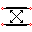
\includegraphics[width=4cm]{coupler}
\end{center}
\caption{ideal coupler device}
\label{fig:coupler}
\end{figure}
\FloatBarrier

The scattering parameters of a coupler are:
\begin{equation}
S_{11} = S_{22} = S_{33} = S_{44} = 0
\end{equation}
\begin{equation}
S_{14} = S_{23} = S_{32} = S_{41} = 0
\end{equation}
\begin{equation}
S_{12} = S_{21} = S_{34} = S_{43} = \sqrt{1-k^2}
\end{equation}
\begin{equation}
S_{13} = S_{31} = S_{24} = S_{42} = k\cdot \exp\left(j\phi\right)
\end{equation}
whereas $0<k<1$ denotes the coupling factor, $\phi$ the phase shift of
the coupling path.  Extending them for an arbitrary reference
impedance $Z_{ref}$, they already become quite complex:

\begin{align}
r &= \dfrac{Z_0-Z_{ref}}{Z_0+Z_{ref}} \\
A &= k^2 \cdot \left( \exp\left(j\cdot 2\phi\right)+1 \right) \\
B &= r^2 \cdot \left(1-A\right) \\
C &= k^2 \cdot \left( \exp\left(j\cdot 2\phi\right)-1 \right) \\
D &= 1 - 2\cdot r^2\cdot \left(1+C\right) + B^2 \\
\end{align}
\begin{equation}
S_{11} = S_{22} = S_{33} = S_{44} = r\cdot\dfrac{A\cdot B + C + 2\cdot r^2\cdot k^2\cdot\exp\left(j\cdot 2\phi\right)}{D}
\end{equation}
\begin{equation}
S_{12} = S_{21} = S_{34} = S_{43} = \sqrt{1-k^2}\cdot \dfrac{\left(1-r^2\right)\cdot \left(1-B\right)}{D}
\end{equation}
\begin{equation}
S_{13} = S_{31} = S_{24} = S_{42} = k\cdot\exp\left(j\phi\right)\cdot \dfrac{\left(1-r^2\right)\cdot \left(1+B\right)}{D}
\end{equation}
\begin{equation}
S_{14} = S_{23} = S_{32} = S_{41} = 2\cdot\sqrt{1-k^2}\cdot k\cdot\exp\left(j\phi\right)\cdot r\cdot \dfrac{\left(1-r^2\right)}{D}
\end{equation}

An ideal coupler is noise free.


\section{Gyrator}

A gyrator is an impedance inverter.  Thus, for example, it converts a
capacitance into an inductance and vice versa.
The ideal gyrator, as shown in fig. \ref{fig:gyrator}, is determined
by the following equations which introduce two more unknowns in the
MNA matrix.

\begin{figure}[ht]
\begin{center}
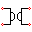
\includegraphics[width=4cm]{gyrator}
\end{center}
\caption{ideal gyrator}
\label{fig:gyrator}
\end{figure}
\FloatBarrier

\begin{equation}
I_{in} = \frac{1}{R}\cdot\left(V_{2} - V_{3}\right)
\quad \rightarrow \quad
\frac{1}{R}\cdot V_{2} - \frac{1}{R}\cdot V_{3} - I_{in} = 0
\end{equation}
\begin{equation}
I_{out} = -\frac{1}{R}\cdot\left(V_{1} - V_{4}\right)
\quad \rightarrow \quad
-\frac{1}{R}\cdot V_{1} + \frac{1}{R}\cdot V_{4} - I_{out} = 0
\label{eq:gyrator}
\end{equation}

The new unknown variables $I_{out}$ and $I_{in}$ must be considered by
the four remaining simple equations.

\begin{equation}
I_{1} = I_{in} \quad I_{2} = I_{out} \quad I_{3} = -I_{out} \quad I_{4} = -I_{in}
\end{equation}

As can be seen, a gyrator consists of two cross-connected VCCS
(section \ref{sec:vccs}). Hence, its y-parameter matrix is:

\begin{equation}
(\underline{Y}) =
\begin{bmatrix}
0&\frac{1}{R}&-\frac{1}{R}&0\\
-\frac{1}{R}&0&0&\frac{1}{R}\\
\frac{1}{R}&0&0&-\frac{1}{R}\\
0&-\frac{1}{R}&\frac{1}{R}&0
\end{bmatrix}
\end{equation}

The scattering matrix
of an ideal gyrator with the ratio $R$ writes as follows.

\begin{equation}
r = \frac{R}{Z_{ref}} = \frac{1}{G\cdot Z_{ref}}
\end{equation}
\begin{equation}
S_{11} = S_{22} = S_{33} = S_{44} = \frac{R^2}{4\cdot Z_{ref}^2 + R^2} = \frac{r^2}{r^2+4}
\end{equation}
\begin{equation}
S_{14} = S_{23} = S_{32} = S_{41} = 1-S_{11}
\end{equation}
\begin{equation}
S_{12} = -S_{13} = -S_{21} = S_{24} = S_{31} = -S_{34} = -S_{42} = S_{43} = \frac{2\cdot r}{r^2+4}
\end{equation}


\section{Voltage and current sources}

For an AC analysis, DC sources are short circuit (voltage source)
and open circuit (current source), respectively. Accordingly,
For a DC analysis, AC sources are short circuit (voltage source)
and open circuit (current source), respectively. As these
sources have no internal resistance, they are noisefree.

\addvspace{12pt}

The MNA matrix of a current source is (with short circuit current $I_0$
flowing into node 1 and out of node 2):

\begin{equation}
\begin{bmatrix}
.&.\\
.&.\\
\end{bmatrix}
\cdot
\begin{bmatrix}
V_{1}\\
V_{2}\\
\end{bmatrix}
=
\begin{bmatrix}
 I_0\\
-I_0\\
\end{bmatrix}
\end{equation}

The MNA matrix of a voltage source is (with open circuit voltage $U_0$
across node 1 to node 2):

\begin{equation}
\begin{bmatrix}
.& .& 1\\
.& .&-1\\
1&-1& 0\\
\end{bmatrix}
\cdot
\begin{bmatrix}
V_{1}\\
V_{2}\\
I_{in}\\
\end{bmatrix}
=
\begin{bmatrix}
 0\\
 0\\
 U_0\\
\end{bmatrix}
\end{equation}

The MNA matrix of a power source is (with internal resistance $R$
and available power $P$):

\begin{equation}
\begin{bmatrix}
 \dfrac{1}{R} & -\dfrac{1}{R} \\
-\dfrac{1}{R} &  \dfrac{1}{R} \\
\end{bmatrix}
\cdot
\begin{bmatrix}
V_{1}\\
V_{2}\\
\end{bmatrix}
=
\begin{bmatrix}
 \sqrt{\dfrac{8\cdot P}{R}}\\
-\sqrt{\dfrac{8\cdot P}{R}}\\
\end{bmatrix}
\end{equation}

The noise current correlation matrix of a power source equals the
one of a resistor with resistance $R$.

\addvspace{12pt}

All voltage sources (AC and DC) are short circuits and therefore their
S-parameter matrix equals the one of the DC block.  All current
sources are open circuits and therefore their S-parameter matrix
equals the one of the DC feed.


\section{Noise sources}

To implement the frequency dependencies of all common noise PSDs the
following equation can be used.

\begin{equation}
PSD = \frac{PSD_0}{a+b\cdot f^c}
\end{equation}

Where $f$ is frequency and $a$, $b$, $c$ are the parameters.  The
following PSDs appear in electric devices.

\addvspace{12pt}

\begin{tabular}{ll}
white noise (thermal noise, shot noise):         & $a=0$, $b=1$, $c=0$ \\
pink noise (flicker noise):                      & $a=0$, $b=1$, $c=1$ \\
Lorentzian PSD (generation-recombination noise): & $a=1$, $b=1/f_c^2$, $c=2$ \\
\end{tabular}


\subsection{Noise current source}

Noise current source with a current power spectral density of $cPSD$:
\begin{equation}
(\underline{C}_Y) = cPSD \cdot
\begin{pmatrix}
 1 & -1 \\
-1 &  1 \\
\end{pmatrix}
\end{equation}

The MNA matrix entries for DC and AC analysis are all zero.

\addvspace{12pt}

The noise wave correlation matrix of a noise current source with
current power spectral density $cPSD$ and its S parameter matrix
write as follows.

\begin{equation}
(\underline{C}) = cPSD\cdot Z_0\cdot
\begin{pmatrix}
   1 & -1\\
  -1 &  1\\
\end{pmatrix}
\qquad
(\underline{S}) =
\begin{pmatrix}
   1 &  0\\
   0 &  1\\
\end{pmatrix}
\end{equation}


\subsection{Noise voltage source}

A noise voltage source (voltage power spectral density $vPSD$) cannot
be modeled with the noise current matrix.  That is why one has to use
a noise current source (current power spectral density $cPSD$)
connected to a gyrator (transimpedance $R$) satisfying the equation
\begin{equation}
vPSD = cPSD \cdot R^2
\end{equation}

Figure \ref{fig:Unoise} shows an example.
\begin{figure}[ht]
\begin{center}
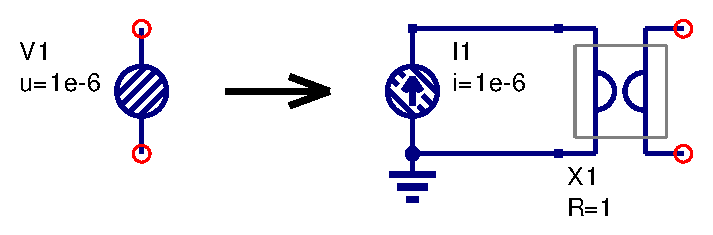
\includegraphics[width=9cm]{Unoise}
\end{center}
\caption{noise voltage source (left-hand side) and its equivalent circuit (right-hand side)}
\label{fig:Unoise}
\end{figure}
\FloatBarrier

The MNA matrix entries of the above construct (gyrator ratio $R=1$) is
similiar to a voltage source with zero voltage.
\begin{equation}
\begin{bmatrix}
.&.& -1\\
.&.& 1\\
1 & -1 & 0
\end{bmatrix}
\cdot
\begin{bmatrix}
V_{1}\\
V_{2}\\
I_x
\end{bmatrix}
=
\begin{bmatrix}
I_{1}\\
I_{2}\\
0
\end{bmatrix}
\end{equation}

The appropriate noise current correlation matrix yields:
\begin{equation}
(\underline{C}_Y) = cPSD \cdot
\begin{pmatrix}
 0 & 0 & 0\\
 0 & 0 & 0\\
 0 & 0 & 1\\
\end{pmatrix}
\end{equation}

The noise wave correlation matrix of a noise voltage source with
voltage power spectral density $vPSD$ and its S parameter matrix
write as follows.

\begin{equation}
(\underline{C}) = \frac{vPSD}{4\cdot Z_0}\cdot
\begin{pmatrix}
   1 & -1\\
  -1 &  1\\
\end{pmatrix}
\qquad
(\underline{S}) =
\begin{pmatrix}
   0 &  1\\
   1 &  0\\
\end{pmatrix}
\end{equation}


\subsection{Correlated noise sources}

For two correlated noise current sources the (normalized) correlation
coefficient $K$ must be known (with $|K|=0\dots 1$). If the first
noise source has the current power spectral
density of $S_{i1}$ and is connected to node 1 and 2, and if furthermore
the second noise source has the spectral density $S_{i2}$ and is connected
to node 3 and 4, then the correlation matrix writes:
\begin{equation}
(\underline{C}_Y) =
\begin{pmatrix}
 S_{i1} & -S_{i1} &  K\cdot\sqrt{S_{i1}\cdot S_{i2}} & -K\cdot\sqrt{S_{i1}\cdot S_{i2}} \\
-S_{i1} &  S_{i1} & -K\cdot\sqrt{S_{i1}\cdot S_{i2}} &  K\cdot\sqrt{S_{i1}\cdot S_{i2}} \\
 K\cdot\sqrt{S_{i1}\cdot S_{i2}} & -K\cdot\sqrt{S_{i1}\cdot S_{i2}} &  S_{i2} & -S_{i2} \\
-K\cdot\sqrt{S_{i1}\cdot S_{i2}} &  K\cdot\sqrt{S_{i1}\cdot S_{i2}} & -S_{i2} &  S_{i2} \\
\end{pmatrix}
\end{equation}

The MNA matrix entries for DC and AC analysis are all zero.

\addvspace{12pt}

The noise wave correlation matrix of two correlated noise current
sources with current power spectral densities $S_{i1}$ and $S_{i2}$
and correlation coefficient $K$ writes as follows.

\begin{equation}
(\underline{C}) = Z_0\cdot
\begin{pmatrix}
 S_{i1} & -S_{i1} &  K\cdot\sqrt{S_{i1}\cdot S_{i2}} & -K\cdot\sqrt{S_{i1}\cdot S_{i2}} \\
-S_{i1} &  S_{i1} & -K\cdot\sqrt{S_{i1}\cdot S_{i2}} &  K\cdot\sqrt{S_{i1}\cdot S_{i2}} \\
 K\cdot\sqrt{S_{i1}\cdot S_{i2}} & -K\cdot\sqrt{S_{i1}\cdot S_{i2}} &  S_{i2} & -S_{i2} \\
-K\cdot\sqrt{S_{i1}\cdot S_{i2}} &  K\cdot\sqrt{S_{i1}\cdot S_{i2}} & -S_{i2} &  S_{i2} \\
\end{pmatrix}
\end{equation}
\begin{equation}
(\underline{S}) =
\begin{pmatrix}
 1 & 0 & 0 & 0 \\
 0 & 1 & 0 & 0 \\
 0 & 0 & 1 & 0 \\
 0 & 0 & 0 & 1 \\
\end{pmatrix}
\end{equation}

For two correlated noise voltage sources two extra
rows and columns are needed in the MNA matrix:

\begin{equation}
\begin{bmatrix}
.&.&.&.& -1 &  0 \\
.&.&.&.&  1 &  0 \\
.&.&.&.&  0 & -1 \\
.&.&.&.&  0 &  1 \\
1 & -1 & 0 &  0 & 0 & 0 \\
0 &  0 & 1 & -1 & 0 & 0 \\
\end{bmatrix}
\cdot
\begin{bmatrix}
V_{1}\\
V_{2}\\
V_{3}\\
V_{4}\\
I_{x1}\\
I_{x2}
\end{bmatrix}
=
\begin{bmatrix}
I_{1}\\
I_{2}\\
I_{3}\\
I_{4}\\
0\\
0
\end{bmatrix}
\end{equation}

The appropriate noise current correlation matrix (with the noise
voltage power spectral densities $S_{v1}$ and $S_{v2}$ and the
correlation coefficient $K$) yields:
\begin{equation}
(\underline{C}_Y) =
\begin{pmatrix}
 0 & 0 & 0 & 0 & 0 & 0\\
 0 & 0 & 0 & 0 & 0 & 0\\
 0 & 0 & 0 & 0 & 0 & 0\\
 0 & 0 & 0 & 0 & 0 & 0\\
 0 & 0 & 0 & 0 & S_{v1} & K\cdot\sqrt{S_{v1}\cdot S_{v2}}\\
 0 & 0 & 0 & 0 & K\cdot\sqrt{S_{v1}\cdot S_{v2}} & S_{v2}\\
\end{pmatrix}
\end{equation}

The noise wave correlation matrix of two correlated noise voltage
sources with voltage power spectral densities $S_{v1}$ and $S_{v2}$
and correlation coefficient $K$ and its S parameter matrix write as
follows.

\begin{equation}
(\underline{C}) = \frac{1}{4\cdot Z_0}\cdot
\begin{pmatrix}
 S_{v1} & -S_{v1} &  K\cdot\sqrt{S_{v1}\cdot S_{v2}} & -K\cdot\sqrt{S_{v1}\cdot S_{v2}} \\
-S_{v1} &  S_{v1} & -K\cdot\sqrt{S_{v1}\cdot S_{v2}} &  K\cdot\sqrt{S_{v1}\cdot S_{v2}} \\
 K\cdot\sqrt{S_{v1}\cdot S_{v2}} & -K\cdot\sqrt{S_{v1}\cdot S_{v2}} &  S_{v2} & -S_{v2} \\
-K\cdot\sqrt{S_{v1}\cdot S_{v2}} &  K\cdot\sqrt{S_{v1}\cdot S_{v2}} & -S_{v2} &  S_{v2} \\
\end{pmatrix}
\end{equation}
\begin{equation}
(\underline{S}) =
\begin{pmatrix}
 0 & 1 & 0 & 0 \\
 1 & 0 & 0 & 0 \\
 0 & 0 & 0 & 1 \\
 0 & 0 & 1 & 0 \\
\end{pmatrix}
\end{equation}


If a noise current source (ports 1 and 2) and a noise voltage
source (ports 3 and 4) are correlated, the MNA matrix entries
are as follows.
\begin{equation}
\begin{bmatrix}
.&.&.&.&  0 \\
.&.&.&.&  0 \\
.&.&.&.& -1 \\
.&.&.&.&  1 \\
0 &  0 & 1 & -1 & 0 \\
\end{bmatrix}
\cdot
\begin{bmatrix}
V_{1}\\
V_{2}\\
V_{3}\\
V_{4}\\
I_x
\end{bmatrix}
=
\begin{bmatrix}
I_{1}\\
I_{2}\\
I_{3}\\
I_{4}\\
0
\end{bmatrix}
\end{equation}

The appropriate noise current correlation matrix (with the noise
power spectral densities $S_{i1}$ and $S_{v2}$ and the
correlation coefficient $K$) yields:
\begin{equation}
(\underline{C}_Y) =
\begin{pmatrix}
 S_{i1} & -S_{i1} & 0 & 0 & K\cdot\sqrt{S_{i1}\cdot S_{v2}}\\
-S_{i1} & S_{i1} & 0 & 0 & 0\\
 0 & 0 & 0 & 0 & 0\\
 0 & 0 & 0 & 0 & 0\\
 K\cdot\sqrt{S_{i1}\cdot S_{v2}} & 0 & 0 & 0 & S_{v2}\\
\end{pmatrix}
\end{equation}
Note: Because the gyrator factor (It is unity.) has been omitted
in the above matrix the units are not correct. This can be ignored.

\addvspace{12pt}

The noise wave correlation matrix of one correlated noise current
source $S_{i1}$ and one noise voltage source $S_{v2}$ with
correlation coefficient $K$ writes as follows.

\begin{equation}
(\underline{C}) =
\begin{pmatrix}
 Z_0\cdot S_{i1} & -Z_0\cdot S_{i1} &  K/2\cdot\sqrt{S_{i1}\cdot S_{v2}} & -K/2\cdot\sqrt{S_{i1}\cdot S_{v2}} \\
-Z_0\cdot S_{i1} &  Z_0\cdot S_{i1} & -K/2\cdot\sqrt{S_{i1}\cdot S_{v2}} &  K/2\cdot\sqrt{S_{i1}\cdot S_{v2}} \\
 K/2\cdot\sqrt{S_{i1}\cdot S_{v2}} & -K/2\cdot\sqrt{S_{i1}\cdot S_{v2}} &  S_{v2}/4/Z_0 & -S_{v2}/4/Z_0 \\
-K/2\cdot\sqrt{S_{i1}\cdot S_{v2}} &  K/2\cdot\sqrt{S_{i1}\cdot S_{v2}} & -S_{v2}/4/Z_0 &  S_{v2}/4/Z_0 \\
\end{pmatrix}
\end{equation}
\begin{equation}
(\underline{S}) =
\begin{pmatrix}
 1 & 0 & 0 & 0 \\
 0 & 1 & 0 & 0 \\
 0 & 0 & 0 & 1 \\
 0 & 0 & 1 & 0 \\
\end{pmatrix}
\end{equation}


\section{Controlled sources}

The models of the controlled sources contain the transfer factor $G$.
It is complex because of the delay time $T$ and frequency $f$.
\begin{equation}
\underline{G} = G\cdot e^{j\omega T} = G\cdot e^{j\cdot 2\pi f\cdot T}
\end{equation}

During a DC analysis (frequency zero) it becomes real because the
exponent factor is unity.


\subsection{Voltage controlled current source}
\label{sec:vccs}

The voltage-dependent current source (VCCS), as shown in fig.
\ref{fig:vccs}, is determined by the following equation which
introduces one more unknown in the MNA matrix.

\begin{figure}[ht]
\begin{center}
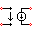
\includegraphics[width=4cm]{vccs}
\end{center}
\caption{voltage controlled current source}
\label{fig:vccs}
\end{figure}
\FloatBarrier

\begin{equation}
I_{out} = G\cdot\left(V_{1} - V_{4}\right)
\quad \rightarrow \quad
V_{1} - V_{4} - \frac{1}{G}\cdot I_{out} = 0
\label{eq:vccs}
\end{equation}

The new unknown variable $I_{out}$ must be considered by the four
remaining simple equations.

\begin{equation}
I_{1} = 0 \quad I_{2} = I_{out} \quad I_{3} = -I_{out} \quad I_{4} = 0
\end{equation}

And in matrix representation this is:
\begin{equation}
\label{eq:vccsStamp}
\begin{bmatrix}
.&.&.&.& 0\\
.&.&.&.& 1\\
.&.&.&.& -1\\
.&.&.&.& 0\\
1 & 0 & 0 & -1 & -\frac{1}{G}
\end{bmatrix}
\cdot
\begin{bmatrix}
V_{1}\\
V_{2}\\
V_{3}\\
V_{4}\\
I_{out}\\
\end{bmatrix}
=
\begin{bmatrix}
I_{1}\\
I_{2}\\
I_{3}\\
I_{4}\\
0\\
\end{bmatrix}
\end{equation}

As you can see the last row which has been added by the VCCS
represents the determining equation (\ref{eq:vccs}).  The additional
right hand column in the matrix keeps the system consistent.

\addvspace{12pt}

When pivotising the above MNA stamp \eqref{eq:vccsStamp} the
additional row and column can be saved ensuring $G$ keeps finite (the
pivot element must be non-zero).  Both representations are equivalent.
If $G$ is zero the below representation must be used.
\begin{equation}
\begin{bmatrix}
0&0&0&0\\
G&0&0&-G\\
-G&0&0&G\\
0&0&0&0
\end{bmatrix}
\cdot
\begin{bmatrix}
V_{1}\\
V_{2}\\
V_{3}\\
V_{4}\\
\end{bmatrix}
=
\begin{bmatrix}
I_{1}\\
I_{2}\\
I_{3}\\
I_{4}\\
\end{bmatrix}
\end{equation}

The scattering matrix of the voltage controlled current source
writes as follows ($\tau$ is time delay).

\begin{equation}
S_{11} = S_{22} = S_{33} = S_{44} = 1
\end{equation}
\begin{equation}
S_{12} = S_{13} = S_{14} = S_{23} = S_{32} = S_{41} = S_{42} = S_{43} = 0
\end{equation}
\begin{equation}
S_{21} = S_{34} = -2\cdot G\cdot \exp\left(-j\omega\tau\right)
\end{equation}
\begin{equation}
S_{24} = S_{31} = 2\cdot G\cdot \exp\left(-j\omega\tau\right)
\end{equation}


\subsection{Current controlled current source}
\label{sec:cccs}

The current-dependent current source (CCCS), as shown in fig.
\ref{fig:cccs}, is determined by the following equation which
introduces one more unknown in the MNA matrix.

\begin{figure}[ht]
\begin{center}
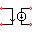
\includegraphics[width=4cm]{cccs}
\end{center}
\caption{current controlled current source}
\label{fig:cccs}
\end{figure}
\FloatBarrier

\begin{equation}
V_{1} - V_{4} = 0
\label{eq:cccs}
\end{equation}

The new unknown variable $I_{out}$ must be considered by the four
remaining simple equations.

\begin{equation}
I_{1} = +\frac{1}{G}\cdot I_{out} \quad I_{2} = I_{out} \quad I_{3} = -I_{out} \quad I_{4} = -\frac{1}{G}\cdot I_{out}
\end{equation}

And in matrix representation this is:
\begin{equation}
\begin{bmatrix}
.&.&.&.& \frac{1}{G}\\
.&.&.&.& 1\\
.&.&.&.& -1\\
.&.&.&.& -\frac{1}{G}\\
1 & 0 & 0 & -1 & 0
\end{bmatrix}
\cdot
\begin{bmatrix}
V_{1}\\
V_{2}\\
V_{3}\\
V_{4}\\
I_{out}\\
\end{bmatrix}
=
\begin{bmatrix}
I_{1}\\
I_{2}\\
I_{3}\\
I_{4}\\
0\\
\end{bmatrix}
\end{equation}

The scattering matrix of the current controlled current source
writes as follows ($\tau$ is time delay).

\begin{equation}
S_{14} = S_{22} = S_{33} = S_{41} = 1
\end{equation}
\begin{equation}
S_{11} = S_{12} = S_{13} = S_{23} = S_{32} = S_{42} = S_{43} = S_{44} = 0
\end{equation}
\begin{equation}
S_{21} = S_{34} = -G\cdot \exp\left(-j\omega\tau\right)
\end{equation}
\begin{equation}
S_{24} = S_{31} = G\cdot \exp\left(-j\omega\tau\right)
\end{equation}


\subsection{Voltage controlled voltage source}
\label{sec:vcvs}

The voltage-dependent voltage source (VCVS), as shown in fig.
\ref{fig:vcvs}, is determined by the following equation which
introduces one more unknown in the MNA matrix.

\begin{figure}[ht]
\begin{center}
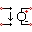
\includegraphics[width=4cm]{vcvs}
\end{center}
\caption{voltage controlled voltage source}
\label{fig:vcvs}
\end{figure}
\FloatBarrier

\begin{equation}
V_{2} - V_{3} = G\cdot \left(V_{1} - V_{4}\right)
\quad \rightarrow \quad
V_{1}\cdot G - V_{2} + V_{3} - V_{4}\cdot G = 0
\label{eq:vcvs}
\end{equation}

The new unknown variable $I_{out}$ must be considered by the four
remaining simple equations.

\begin{equation}
I_{1} = 0 \quad I_{2} = -I_{out} \quad I_{3} = I_{out} \quad I_{4} = 0
\end{equation}

And in matrix representation this is:
\begin{equation}
\begin{bmatrix}
.&.&.&.& 0\\
.&.&.&.& -1\\
.&.&.&.& 1\\
.&.&.&.& 0\\
G & -1 & 1 & -G & 0
\end{bmatrix}
\cdot
\begin{bmatrix}
V_{1}\\
V_{2}\\
V_{3}\\
V_{4}\\
I_{out}\\
\end{bmatrix}
=
\begin{bmatrix}
I_{1}\\
I_{2}\\
I_{3}\\
I_{4}\\
0\\
\end{bmatrix}
\end{equation}

The scattering matrix of the voltage controlled voltage source
writes as follows ($\tau$ is time delay).

\begin{equation}
S_{11} = S_{23} = S_{32} = S_{44} = 1
\end{equation}
\begin{equation}
S_{12} = S_{13} = S_{14} = S_{22} = S_{33} = S_{41} = S_{42} = S_{43} = 0
\end{equation}
\begin{equation}
S_{21} = S_{34} = G\cdot \exp\left(-j\omega\tau\right)
\end{equation}
\begin{equation}
S_{24} = S_{31} = -G\cdot \exp\left(-j\omega\tau\right)
\end{equation}


\subsection{Current controlled voltage source}
\label{sec:ccvs}

The current-dependent voltage source (CCVS), as shown in fig.
\ref{fig:ccvs}, is determined by the following equations which
introduce two more unknowns in the MNA matrix.

\begin{figure}[ht]
\begin{center}
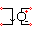
\includegraphics[width=4cm]{ccvs}
\end{center}
\caption{current controlled voltage source}
\label{fig:ccvs}
\end{figure}
\FloatBarrier

\begin{equation}
V_{1} - V_{4} = 0
\end{equation}
\begin{equation}
V_{2} - V_{3} = G\cdot I_{in}
\quad \rightarrow \quad
V_{2} - V_{3} - I_{in}\cdot G = 0
\label{eq:ccvs}
\end{equation}

The new unknown variables $I_{out}$ and $I_{in}$ must be considered by
the four remaining simple equations.

\begin{equation}
I_{1} = I_{in} \quad I_{2} = -I_{out} \quad I_{3} = I_{out} \quad I_{4} = -I_{in}
\end{equation}

The matrix representation needs to be augmented by two more new rows
(for the new unknown variables) and their corresponding columns.
\begin{equation}
\begin{bmatrix}
.&.&.&.& 1 & 0\\
.&.&.&.& 0 & -1\\
.&.&.&.& 0 & 1\\
.&.&.&.& -1 & 0\\
0 & 1 & -1 & 0 & -G & 0\\
1 & 0 & 0 & -1 & 0 & 0
\end{bmatrix}
\cdot
\begin{bmatrix}
V_{1}\\
V_{2}\\
V_{3}\\
V_{4}\\
I_{in}\\
I_{out}
\end{bmatrix}
=
\begin{bmatrix}
I_{1}\\
I_{2}\\
I_{3}\\
I_{4}\\
0\\
0
\end{bmatrix}
\end{equation}

The scattering matrix of the current controlled voltage source
writes as follows ($\tau$ is time delay).

\begin{equation}
S_{14} = S_{23} = S_{32} = S_{41} = 1
\end{equation}
\begin{equation}
S_{11} = S_{12} = S_{13} = S_{22} = S_{33} = S_{42} = S_{43} = S_{44} = 0
\end{equation}
\begin{equation}
S_{21} = S_{34} = \frac{G}{2}\cdot \exp\left(-j\omega\tau\right)
\end{equation}
\begin{equation}
S_{24} = S_{31} = -\frac{G}{2}\cdot \exp\left(-j\omega\tau\right)
\end{equation}


\section{Transmission Line}
\label{sec:tl_yparameter}

A transmission line is usually described by its ABCD-matrix.  (Note
that in ABCD-matrices, i.e. the chain matrix representation, the
current $i_2$ is defined to flow out of the output port.)
\begin{equation}
\label{eq:tl_apara}
\left(\underline{A}\right) =
\begin{pmatrix}
\cosh{\left(\gamma\cdot l\right)} & Z_L\cdot \sinh{\left(\gamma\cdot l\right)}\\
\sinh{\left(\gamma\cdot l\right)} / Z_L & \cosh{\left(\gamma\cdot l\right)}
\end{pmatrix}
\end{equation}

These can easily be recalculated into impedance parameters.
\begin{align}
Z_{11} = Z_{22} &= \frac{Z_L}{\tanh{\left(\gamma\cdot l\right)}}\\
Z_{12} = Z_{21} &= \frac{Z_L}{\sinh{\left(\gamma\cdot l\right)}}
\end{align}

Or in admittance parameter representation it yields
\begin{equation}
\label{eq:TransLineY}
\begin{split}
Y_{11} = Y_{22} &= \frac{1}{Z_L \cdot \tanh{\left(\gamma\cdot l\right)}}\\
Y_{12} = Y_{21} &= \frac{-1}{Z_L\cdot \sinh{\left(\gamma\cdot l\right)}}
\end{split}
\end{equation}

whence $\gamma$ denotes the propagation constant $\alpha + j\beta$ and
$l$ is the length of the transmission line.  $Z_L$ represents the
characteristic impedance of the transmission line.  The Y-parameters
as defined by eq. \eqref{eq:TransLineY} can be used for the microstrip
line.  For an ideal, i.e. lossless, transmission lines they write
accordingly.
\begin{align}
Z_{11} = Z_{22} &= \frac{Z_L}{j\cdot\tan{\left(\beta\cdot l\right)}}\\
Z_{12} = Z_{21} &= \frac{Z_L}{j\cdot\sin{\left(\beta\cdot l\right)}}\\
Y_{11} = Y_{22} &= \frac{1}{j\cdot Z_L \cdot \tan{\left(\beta\cdot l\right)}}\\
Y_{12} = Y_{21} &= \frac{j}{Z_L\cdot \sin{\left(\beta\cdot l\right)}}
\end{align}

The scattering matrix of an ideal, lossless transmission line with
impedance $Z$ and electrical length $l$ writes as follows.

\begin{equation}
r = \frac{Z-Z_0}{Z+Z_0}
\end{equation}
\begin{equation}
p = \exp\left(-j\omega\frac{l}{c_0}\right)
\end{equation}
\begin{equation}
S_{11} = S_{22} = \frac{r\cdot(1-p^2)}{1-r^2\cdot p^2} \qquad,\qquad
S_{12} = S_{21} = \frac{p\cdot(1-r^2)}{1-r^2\cdot p^2}
\end{equation}

With $c_0$ = 299 792 458 m/s being the vacuum light velocity.
Adding attenuation to the transmission line, the quantity $p$
extends to:
\begin{equation}
p = \exp\left(-j\omega\frac{l}{c_0} - \alpha\cdot l \right)
\end{equation}

Another equivalent equation set for the calculation of the
scattering parameters is the foolowing:
With the physical length $l$ of the component, its impedance
$Z_L$ and propagation constant $\gamma$, the complex propagation
constant $\gamma$ is given by
\begin{equation}
\gamma = \alpha + j\beta
\end{equation}

where $\alpha$ is the attenuation factor and $\beta$ is the (real)
propagation constant given by
\begin{equation}
\beta = \sqrt{\varepsilon_{r_{eff}}(\omega)} \cdot k_0
\end{equation}

where $\varepsilon_{r_{eff}}(\omega)$ is the effective dielectric
constant and $k_0$ is the TEM propagation constant $k_0$ for the
equivalent transmission line with an air dielectric.
\begin{equation}
k_0 = \omega \sqrt{\varepsilon_0 \mu_0}
\end{equation}

The expressions used to calculate the scattering parameters are given
by
\begin{align}
S_{11} = S_{22} &= \dfrac{\left(z - y\right) \sinh{\gamma l}}{2\cosh{\gamma l} + \left(z + y\right) \sinh{\gamma l}}\\
S_{12} = S_{21} &= \dfrac{2}{2\cosh{\gamma l} + \left(z + y\right) \sinh{\gamma l}}
\end{align}

with $z$ being the normalized impedance and $y$ is the normalized
admittance.


\section{Coupled transmission line}
\label{sec:coupledtline}

A coupled transmission line is described by two identical transmission
line ABCD-matrices, one for the even and one for the odd mode.
Because the coupled lines are a symmetrical 3-line system, the
matrices are completely independent of each other.  Therefore, its
Y-parameters write as follows.
\begin{align}
Y_{11} = Y_{22} = Y_{33} = Y_{44} &= \frac{1}{2\cdot Z_{L,e} \cdot \tanh\left(\gamma_e\cdot l\right)}
              + \frac{1}{2\cdot Z_{L,o} \cdot \tanh\left(\gamma_o\cdot l\right)}\\
Y_{12} = Y_{21} = Y_{34} = Y_{43} &= \frac{-1}{2\cdot Z_{L,e} \cdot \sinh\left(\gamma_e\cdot l\right)}
              + \frac{-1}{2\cdot Z_{L,o} \cdot \sinh\left(\gamma_o\cdot l\right)}\\
Y_{13} = Y_{31} = Y_{24} = Y_{42} &= \frac{-1}{2\cdot Z_{L,e} \cdot \sinh\left(\gamma_e\cdot l\right)}
              + \frac{1}{2\cdot Z_{L,o} \cdot \sinh\left(\gamma_o\cdot l\right)}\\
Y_{14} = Y_{41} = Y_{23} = Y_{32} &= \frac{1}{2\cdot Z_{L,e} \cdot \tanh\left(\gamma_e\cdot l\right)}
              + \frac{-1}{2\cdot Z_{L,o} \cdot \tanh\left(\gamma_o\cdot l\right)}
\end{align}

The S-parameters (according to the port numbering in
fig. \ref{fig:mscoupled}) are as followed \cite{Edwards}.

\addvspace{12pt}

reflection coefficients
\begin{equation}
S_{11} = S_{22} = S_{33} = S_{44} = X_e + X_o
\end{equation}
through paths
\begin{equation}
S_{12} = S_{21} = S_{34} = S_{43} = Y_e + Y_o
\end{equation}
coupled paths
\begin{equation}
S_{14} = S_{41} = S_{23} = S_{32} = X_e - X_o
\end{equation}
isolated paths
\begin{equation}
S_{13} = S_{31} = S_{24} = S_{42} = Y_e - Y_o
\end{equation}

with the denominator
\begin{equation}
D_{e,o} = 2\cdot Z_{L,e,o}\cdot Z_0\cdot \cosh(\gamma_{e,o}\cdot l)
         + \left(Z_{L,e,o}^2 + Z_0^2\right)\cdot \sinh\left(\gamma_{e,o}\cdot l\right)
\end{equation}

and
\begin{align}
X_{e,o} &= \frac{\left(Z_{L,e,o}^2 - Z_0^2\right)\cdot \sinh\left(\gamma_{e,o}\cdot l\right)}{2\cdot D_{e,o}}\\
Y_{e,o} &= \frac{Z_{L,e,o}\cdot Z_0}{D_{e,o}}
\end{align}

\begin{figure}[ht]
\begin{center}
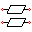
\includegraphics[width=0.5\linewidth]{mscoupled}
\end{center}
\caption{coupled transmission line}
\label{fig:mscoupled}
\end{figure}
\FloatBarrier


\section{S-parameter container with additional reference port}
\label{sec:spfile}

The Y-parameters of a multi-port component defined by its S-parameters
required for a small signal AC analysis can be obtained by converting
the S-parameters into Y-parameters.

\begin{figure}[ht]
\begin{center}
\includegraphics[width=0.6\linewidth]{spnfile}
\end{center}
\caption{S-parameter container with noise wave correlation matrix}
\label{fig:spnfile}
\end{figure}
\FloatBarrier

In order to extend a $m - 1$-port to have a S-parameter device with
$m$ ports assuming that the original reference port had a reflection
coefficient $\Gamma_m$ the new S-parameters are according to
T. O. Grosch and L. A. Carpenter \cite{Grosch}:
\begin{align}
S_{mm} &= \dfrac{2 - \Gamma_m - m + {\displaystyle\sum_{i=1}^{m-1}}\, {\displaystyle\sum_{j=1}^{m-1}} S'_{ij}}{1 - m\cdot \Gamma_m - {\displaystyle\sum_{i=1}^{m-1}}\, {\displaystyle\sum_{j=1}^{m-1}} S'_{ij}}\\
S_{im} &= \left(\dfrac{1 - \Gamma_m\cdot S_{mm}}{1 - \Gamma_m}\right)\cdot \left(1 - \sum_{j=1}^{m-1} S'_{ij}\right) &
\textrm{ for } i = 1,2 \ldots m - 1\\
S_{mj} &= \left(\dfrac{1 - \Gamma_m\cdot S_{mm}}{1 - \Gamma_m}\right)\cdot \left(1 - \sum_{i=1}^{m-1} S'_{ij}\right) &
\textrm{ for } j = 1,2 \ldots m - 1\\
S_{ij} &= S'_{ij} - \left(\dfrac{\Gamma_m\cdot S_{im}\cdot S_{mj}}{1 - \Gamma_m\cdot S_{mm}}\right) &
\textrm{ for } i,j = 1,2 \ldots m - 1
\end{align}

If the reference port has been ground potential, then $\Gamma_m$
simply folds to -1.  The reverse transformation by connecting a
termination with a reflection coefficient of $\Gamma_m$ to the $m$th
port writes as follows.
\begin{equation}
S'_{ij} = S_{ij} + \left(\dfrac{\Gamma_m\cdot S_{im}\cdot S_{mj}}{1 - \Gamma_m\cdot S_{mm}}\right)
\;\;\;\; \textrm{ for } i,j = 1,2 \ldots m - 1
\end{equation}

With the S-parameter transformation done the $m$-port noise wave
correlation matrix is
\begin{equation}
C_m = \left|\dfrac{1}{1 - \Gamma_m}\right|^2 \cdot \left(K\cdot C_{m-1}\cdot K^+ -T_s\cdot k_B \cdot\left|1 - \left|\Gamma_m\right|^2\right|\cdot D\cdot D^+\right)
\end{equation}

with
\begin{align}
K &=
\begin{bmatrix}
1 + \Gamma_m\left(S_{1m} -1\right) & \Gamma_m S_{1m} & \ldots & \Gamma_m S_{1m}\\
\Gamma_m S_{2m} & 1 + \Gamma_m\left(S_{2m} -1\right) & \ldots & \Gamma_m S_{2m}\\
\vdots & \vdots & \ddots & \vdots\\
\Gamma_m S_{(m-1)m} & \Gamma_m S_{(m-1)m} & \ldots & 1 + \Gamma_m\left(S_{(m-1)m} -1\right)\\
\Gamma_m S_{mm} - 1 & \Gamma_m S_{mm} - 1 & \ldots & \Gamma_m S_{mm} - 1
\end{bmatrix}\\
D &=
\begin{bmatrix}
S_{1m}\\
S_{2m}\\
\vdots\\
S_{(m-1)m}\\
S_{mm} - 1
\end{bmatrix}
\end{align}

whence $T_s$ denotes the equivalent noise temperature of the original
reference port and the $ ^{+}$ operator indicates the transposed
conjugate matrix (also called adjoint or adjugate).

\addvspace{12pt}

The reverse transformation can be written as
\begin{equation}
C_{m-1} = K'\cdot C_m\cdot K'^+ +T_s\cdot k_B \cdot\dfrac{\left|1 - \left|\Gamma_m\right|^2\right|}{\left|1 - \Gamma_m S_{mm}\right|^2}\cdot D'\cdot D'^+
\end{equation}

with
\begin{align}
K' &=
\begin{bmatrix}
1 & 0 & \ldots & 0 & \dfrac{\Gamma_m S_{1m}}{1 - \Gamma_m S_{mm}}\\
0 & 1 & \ldots & 0 & \dfrac{\Gamma_m S_{2m}}{1 - \Gamma_m S_{mm}}\\
. & . & \ddots & . & \vdots\\
0 & 0 & \ldots & 1 & \dfrac{\Gamma_m S_{(m-1)m}}{1 - \Gamma_m S_{mm}}\\
\end{bmatrix}\\
D' &=
\begin{bmatrix}
S_{1m}\\
S_{2m}\\
\vdots\\
S_{(m-1)m}
\end{bmatrix}
\end{align}
